\documentclass{article}
  \usepackage[utf8]{inputenc}
  \usepackage{mathtools}
  \usepackage{listings}
  \usepackage{graphicx}
  \usepackage{url}
  \title{The on-chain claiming mechanism economics}
  \author{Piotr Kosiński\thanks{Thanks to Vijay Kandy, Piper Merriam, Logan Saether for the contribution.}\\ChronoLogic}
  \date{\today\\v1.0}
  \begin{document}
  \maketitle
  \begin{abstract}
    Running a service like a TimeNode can be profitable for the operators, however, given the many variables that influence its payout,  it's not trivial to estimate the expected profits. The proposed model and simulation code has been created to address that problem.
  \end{abstract}
  \section{Introduction}
  This article describes the economic model for on-chain claiming mechanism used by the Ethereum Alarm Clock protocol. This mechanism has been implemented in order to improve the economics of running the \textbf{TimeNode}\footnote{TimeNode is an off-chain executing agent that scans the blockchain for new scheduled transactions and attempts the execution}. 
  
  Given that scheduled transactions are expected to be executed at the exact time and the network of $n$ competing nodes exists, we expect to face the "swarming" problem which can be described as: \textit{uncoordinated attempts of execution by $n$ nodes at the same time}. This problem may result in unnecessary costs\footnote{due to the fact that all transactions on the Ethereum network costs gas, successful and failed} for \textbf{TimeNode} making the operations potentially not profitable as only 1-of-$n$ is going to earn the TimeBounty for the execution, other \textbf{TimeNodes} trying to execute at the same block will pay the failing transaction cost.
  
  By introducing payment modifier $P_{mod}$ \textbf{TimeNode} operators are able to pick theirs profitability point, this effectively allows to mitigate the "swarming" problem as we expect \textbf{TimeNodes} to try to claim on different blocks/moment of time. 
  \section{Claiming mechanism}
  Claiming mechanism can be described as follows:
  For any transaction $Tx$ that has been deployed to the network and is expected to be executed by 1 of $n$ nodes in the network. The process of execution is divided into two steps:
  \textbf{claiming} and \textbf{execution}. Claiming is a process of reserving the transaction for further execution.
  \begin{figure}
    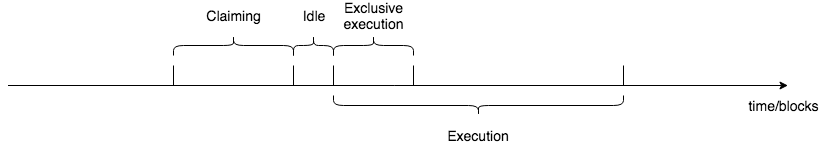
\includegraphics[width=\linewidth]{timeranges.png}
    \caption{Scheduled transaction life cycle}
    \label{fig:boat1}
  \end{figure}
  
  \subsection{Claiming}
  \begin{itemize}
  \item can happen before execution
  \item every node has the same chance to successfully claim $Tx$
  \item claiming requires a $Deposit$ to be locked by claimant
  \item $Deposit$ is lost by claimant when execution won't happen within \textit{exclusive execution window}
  \item every node can fail on claiming when $Tx$ was already claimed
  \item claiming requires sending transaction that has cost described as $C_{c}$ when success and $C_{f}$ when failure
  \item payment modifier $P_{mod}(t)=\begin{cases}
  0 & \quad \text{at beginning of claiming window}\\
  1 & \quad \text{at end of claiming window}
  \end{cases}$ 
  \item claiming is optional
  \end{itemize}
  
  \subsection{Execution}
  \begin{itemize}
  \item successful execution has reward described as $TimeBounty$ 
  \item execution cost is reimbursed by the scheduler when successful
  \item execution cost has cost described as $C_{e}$ when not successful
  \item $Deposit$ locked by the claimant can be acquired by a node when the claimant failed to execute
  \end{itemize}
  
  \subsection{Expected payout definition}
  Let's define the expected payout for node as
  \[
  P=P_{s}+P_{f}+P_{nf}
  \]
  where
  \\
  
  $P_{s}$ is expected payout after successful claiming and execution
  \\
  
  $P_{f}$ is expected payout after successful claiming and missed execution
  \\
  
  $P_{nf}$ is expected payout after other node losing the deposit
  \\
  
  \subsubsection{Network with $n=1$ nodes}
  For network of nodes with $n=1$ we can define expected payouts as:
  \[
  P_{s}(P_{mod})=P_{mod} \times TimeBounty-C_{C} 
  \]
  \[
  P_{f}=-C_{C}-Deposit
  \]
  \[
  P_{nf}=TimeBounty-C_{C}
  \]
  \subsubsection{Network with $n>1$ nodes}
  For that case the expected reward will be $\frac{TimeBounty}{n}$ assuming that probability of successful claiming is equal for all nodes. Also in case of failing transaction node will pay the $C_{Tx}$
  \[
  P_{s}(P_{mod})=\frac{P_{mod} \times TimeBounty-C_{C}}{n} - (n-1) \times C_{Tx}
  \]
  \[
  P_{f}=-C_{C}-Deposit
  \]
  \[
  P_{nf}=\frac{TimeBounty-C_{C}}{n} - (n-1) \times C_{Tx}
  \]
  
  In order to improve the cost of failing transactions let's introduce a mechanism $X$ that prevents sending the transaction that will fail, the accuracy of mechanism $X$ is defined as $A_{X} \in [0;1]$
  
  \[
  P_{s}(A_{X}, P_{mod})=\frac{P_{mod} \times TimeBounty-C_{C}}{n} - (1-A_{X}) \times (n-1) \times C_{Tx}
  \]
  \[
  P_{f}=-C_{C}-Deposit
  \]
  \[
  P_{nf}(A_{X})=\frac{TimeBounty-C_{C}}{n} - (1-A_{X}) \times (n-1) \times C_{Tx}
  \]
  
  The last part is to introduce $P_{ld} \in [0;1]$ as probability of TimeNode loosing the $Deposit$
  
  
  \[
  \label{eq}
  P(A_{X}, P_{ld}, P_{mod})=P_{s}(A_{X}, P_{mod}) \times (1-P_{ld}) + (P_{f}(A_{X})+P_{nf}(A_{X})) \times P_{ld}
  \]
  \section{Simulation}
  We are going to simulate few cases using equation formulated in section \ref{eq}. $A_{X}, P_{ld}, P_{mod}$ are the variables that depends on reliability and running costs by TimeNode owners. All calculated results are going to be represented as \textit{gas}
  
  Let' now define the profitability threshold, we assume monthly running cost for the TimeNode is 7USD (this is based on current rates on Heroku cloud). Translating 7USD to \textit{gas} we get:
  
  \begin{align*}
  ETH/USD=700USD\\
  Gas Price = 10Gwei\\
  7USD \equiv 1000000gas
  \end{align*}
  
  This shows us that running costs are covered after acquiring 1000000\textit{gas}. Now let's take a look at how this translates to the amount of executed transactions. In order to calculate $P(A_{X}, P_{ld}, P_{mod})$ we use the script listed below. More over we are using these values describing TimeNode operations and network conditions.
  \begin{align*}
  &n \approx 8\\
  &TimeBounty \approx 300000gas\\
  &Deposit \approx 600000gas\\
  &A_{X} \approx 0.95 (95\%)\\
  &P_{ld} \approx 0.1 (1\%)\\
  &C_{C} = 90000gas\\
  &C_{Tx} = 25000gas\\
  &target = 1000000gas~or~7USD
  \end{align*}
  Results using these parameters are:
  \begin{verbatim}
     p_mod      res num_of_tx
  16  0.75 1164.673       858
  17  0.80 2442.108       409
  18  0.85 3957.999       252
  19  0.90 5381.834       185
  20  0.95 6967.551       143
  21  1.00 8388.889       119
  \end{verbatim}
  Results data frame contains 3 columns:
  \begin{itemize}
  \item \textbf{p\_mod} - payment modifier ($P_{mod}$)
  \item \textbf{res} - expected amount of gas earned by TimeNode per transaction
  \item \textbf{num\_of\_tx} - number of transactions to be executed in order to cover running costs
  \end{itemize}
  
  The results achieved by running this simulation should be treated informational rather than something taken for granted. The expected payout depends on all of the variables described above, for a simulation purpose we picked values using our intuition.
  
  The variable controlled by the TimeNode operator is $P_{mod}$ which is the major component. Low enough $P_{mod}$ allows TimeNode to claim transaction before others, still, in order to be profitable using low $P_{mod} $, the TimeNode running cost has to be low.     
  
  The TimeNode market has many characteristics of the perfect competition market\footnote{\url{http://www.economicsonline.co.uk/Business_economics/Perfect_competition.html}}: there is perfect information, no barriers to entry, they deliver the same service, TimeNode are the price takers. Based on that, long-term we may get in the situation where marginal cost is equal average cost. 
  \appendix
  \section{Simulation source code}
  \lstinputlisting[language=R, caption=Siml.R]{onchain_claiming_mechanism.R}
  
  \end{document}
  